\documentclass{article}
\usepackage[utf8]{inputenc}
\usepackage{amsthm}
\usepackage{amsmath, mathtools, amsfonts,amssymb}
\usepackage{graphicx}
\usepackage{verbatim}
\usepackage{fancyhdr}

\usepackage{subfigure}
% Code
\usepackage{listings} 
\usepackage{algorithm}
\usepackage{algpseudocode}
\usepackage{float}
% Margins
\usepackage{geometry}
%\geometry{margin=1in} %% 
% Graphics
\usepackage{tikz}
\usetikzlibrary{matrix} % matrices
\usepackage{tikz-qtree} % Simple trees
\usepackage{hyperref} % hyperlinks
% Theorems/etc.
\newtheorem{pic}{Figure}
\numberwithin{pic}{section}
\newtheorem{lem}{Lemma}
\numberwithin{lem}{section}
\newtheorem{thm}{Theorem}
\numberwithin{thm}{section}
\newtheorem{cor}{Corollary}
\numberwithin{cor}{section}
\theoremstyle{definition}
\newtheorem{ex}{Example}
\numberwithin{ex}{section}
\newtheorem{defn}{Definition}
\numberwithin{defn}{section}
\theoremstyle{definition}
\newtheorem{prob}{Problem}
\theoremstyle{remark}
\newtheorem*{con}{Conjecture}
\newtheorem{rem}{Remark}
\newtheorem*{cex}{Counterexample}
\newtheorem*{ts}{T.S.}


%%% COMMANDS %%%
% Sets
\newcommand{\set}[1]{\ensuremath{\left\{ #1\right\}}} % write sets
\newcommand{\e}{\ensuremath{\epsilon}} % Epsilon
\newcommand{\R}{\ensuremath{\mathbb{R}}} % Real Numbers
\newcommand{\C}{\ensuremath{\mathbb{C}}} % Complex Numbers
\newcommand{\N}{\ensuremath{\mathbb{N}}} % Natural numbers
\newcommand{\Q}{\ensuremath{\mathbb{Q}}} % Rationals
\newcommand{\I}{\ensuremath{\mathbb{I}}} % Irrational Numbers
\newcommand{\Z}{\ensuremath{\mathbb{Z}}} % Integers
% Easier Delimiters?
\newcommand{\lr}[2]{\ensuremath{\left#1 #2 \right #1}}
% Absolute Value
\newcommand{\abs}[1]{\ensuremath{\left| #1 \right|}}
% Landau Notation
\newcommand{\Oh}{\ensuremath{\mathcal{O}}} %%% IN MATH MODE
\newcommand{\oh}{\ensuremath{\mathcal{o}}} %%% IN MATH MODE
% Display style fractions
\newcommand{\Frac}[2]{\displaystyle \frac{#1}{#2}}
% Display style limits
\newcommand{\Lim}[2]{\displaystyle \lim_{#1}{#2}}

%% Norms %%
\newcommand{\norm}[1]{\ensuremath{\left | \left | #1 \right | \right |}}
%%% Preference Stuff %%%
\setcounter{section}{-1}
\renewcommand\qedsymbol{{$\blacksquare$}}
% Enumerate
\renewcommand{\labelenumi}{(\alph{enumi})}
\renewcommand{\labelenumii}{\roman{enumii}}
% change proof environment
\renewcommand*{\proofname}{Pf}
% Line Spacing
\renewcommand{\baselinestretch}{1.5}
% Indentation
\newlength\tindent
\setlength{\tindent}{\parindent}
\setlength{\parindent}{0pt}
\renewcommand{\indent}{\hspace*{\tindent}}
% Set title
\title{Computational Math Project\\
  {\large Illinois Institute of Technology}
}
\author{
  Miles Bakenhus 
  \and
  Ahmed Lodhika 
  \and
  Gunjan Sharma 
  \and
  Quinn Stratton 
  \and
  Jan-Eric Sulzbach 
}
\date{\today}
\begin{document}
\fancyhead[l]{}
\fancyhead[c]{}
\fancyhead[r]{}
% \pagestyle{fancy}
\maketitle
\newpage
\tableofcontents
\section{Introduction}
\indent In this paper we discuss what motivates the study of banded matrices and show several results regarding their properties. We will also consider the application of these properties to find a more efficient implementation of the Modified Gram-Schmidt Algorithm. Finally, we will discuss potential future work.
\section{Origin of the problem and its applications}
\paragraph{} In this part of the project we explain the motivation behind our ideas and examine the applications of our results. First, we consider the standard elliptic equation in two dimensions
\begin{align*}
-\Delta u &= f ~\text{ in } \Omega\\
u&=0 ~\text{ on } \partial\Omega.
\end{align*}
Then the discretised equation on a grid is
\begin{align*}
-\Delta_h u_{ij} &= f_{ij} ~\forall\,(x_i,y_i)\in \Omega_h,~f_{ij}=f(x_i,y_j)\\
u_{ij}&=0 ~\forall\,(x_i,y_i)\in \partial\Omega_h,
\intertext{where we use the second-order central differencing to represent the Laplace operator}
-\Delta_h u_{ij}= \Frac 1{h^2}\begin{pmatrix}
0 & -1 & 0 \\ 
-1 & 4 & -1 \\ 
0 & -1 & 0
\end{pmatrix}u_{ij}&= \Frac 1{h^2} \big(-u_{ij+1}-u_{i-1j}+4 u_{ij}-u_{i+1j}-u_{ij_1}\big)
\end{align*}
If we assume that the domain $\Omega$ is a square, ordering the grid points from left to right and bottom to top yields the following matrix of the system $A\in \R^{(h-1)^{-2}\times (h-1)^{-2}}$:
\[A=h^2\begin{pmatrix}
4 & -1 & 0 & \dots & 0 & -1 &  &  \\ 
-1 & 4 & -1 &  &  &  & \ddots &  \\ 
0 & -1 & 4 & \ddots &  &  &  & -1 \\ 
\vdots  &  & \ddots & \ddots &  &  &  & 0\\ 
0 &  &  &  &  &  &  & \vdots \\ 
-1 &  &  &  &  & \ddots & \ddots & 0 \\ 
 & \ddots &  &  &  & \ddots & 4 & -1 \\ 
 &  & -1 & 0 & \dots & 0 & -1 & 4
\end{pmatrix} \]
And, the problem we need to solve is the linear system $Au=f$.\\
\indent Therefore, it is important to understand how the structure of $A$ affects the structure of the $QR$ decomposition.
Note that in this case the highest and lowest off-diagonal has a distance of order $h$ from the diagonal.

\paragraph{} Another example where these banded matrices show up is in the following:
consider the parabolic equation in two dimensions
\[\frac{\partial u}{\partial t}=\sigma \Delta u,~ 0\leq x\leq X,\, 0\leq y\leq Y\, 0\leq t\leq T\]
with Dirichlet boundary condition and given initial data $u(x,y,0)=U^0(x,y)$. For the numerical implementation we consider the implicit Crank-Nicolson scheme
\begin{align*}
&-\frac{\mu_x}{2}\big(U_{j-1,l}^{n+1}+ U_{j+1,l}^{n+1}\big) -\frac{\mu_y}{2}\big(U_{j,l-1}^{n+1}+U_{j,l+1}^{n+1}\big)+\big(1+\mu_x+\mu_y\big)U_{j,l}^{n+1}\\
=&\frac{\mu_x}{2}\big(U_{j-1,l}^{n}+ U_{j+1,l}^{n}\big) +\frac{\mu_y}{2}\big(U_{j,l-1}^{n}+U_{j,l+1}^{n}\big)+\big(1-\mu_x-\mu_y\big)U_{j,l}^{n},
\end{align*}
for $0\leq j\leq J_x$, $0\leq l\leq J_y$ and $n>0$.
Again, we can rewrite this as a linear system $AU^{n+1}=U^n$, with 
\[A=\begin{pmatrix}
1+\mu_x+\mu_y & -\frac{\mu_x}{2} & 0 & \dots & 0 & -\frac{\mu_y}{2} &  &  \\ 
-\frac{\mu_x}{2} & 1+\mu_x+\mu_y & -\frac{\mu_x}{2} &  &  &  & \ddots &  \\ 
0 & -\frac{\mu_x}{2} & 1+\mu_x+\mu_y & \ddots &  &  &  & -\frac{\mu_y}{2} \\ 
\vdots  &  & \ddots & \ddots &  &  &  & 0\\ 
0 &  &  &  &  &  &  & \vdots \\ 
-\frac{\mu_y}{2} &  &  &  &  & \ddots & \ddots & 0 \\ 
 & \ddots &  &  &  & \ddots & 1+\mu_x+\mu_y & -\frac{\mu_x}{2} \\ 
 &  & -\frac{\mu_y}{2} & 0 & \dots & 0 & -\frac{\mu_x}{2} & 1+\mu_x+\mu_y
\end{pmatrix} \]
and $A\in\R^{(J_x-1)(J_y-1)\times (J_x-1)(J_y-1)}$ where the highest and lowest off-diagonal band have the distance $J_x-1$ from the diagonal.
\begin{rem}
In the case of three dimension, we would obtain one more non-zero sub/super-diagonal, now with a distance of $\mathcal{O}(J_x*J_y)$ from the diagonal.
\end{rem}
\pagebreak
\section{Matrix Properties}
\subsection{Tridiagonal Matrices}
\begin{thm}
If $A$ is a tridiagonal matrix, then R in the product $A=QR$ is an upper triangular matrix with non-zero entries only in the diagonal and first two superdiagonals.
\end{thm}
\[A=\begin{pmatrix}
a_{11} & a_{12} &  &   \\ 
a_{21} & a_{22} & a_{23} &    \\ 
 & \ddots & \ddots & \ddots   \\ 
   &  & a_{m m-1} & a_{mm}
\end{pmatrix}~,~R=\begin{pmatrix}
r_{11} & r_{12} & r_{13} &  \\ 
 & \ddots & \ddots & \ddots \\ 
 &  & \ddots & \ddots \\ 
 &  &  & r_{mm}
\end{pmatrix}  \]
\begin{proof}
To prove the statement we will use the classical Gram-Schmidt (CGS) method for the QR decomposition.\\ 
Step 1: show that $q_j$ has the form $q_j=\begin{pmatrix}
* \\ 
\vdots \\ 
* \\ 
0 \\ 
\vdots
\end{pmatrix} \leftarrow j+1\text{-th entry}$.\\
We prove this by induction:
\begin{description}
\item[Base step:] For $j=1$, if we assume that $\|a_1\|=1$, then $q_1=a_1$. Thus
\[q_1= \begin{pmatrix}
a_{11} \\ 
a_{21} \\ 
0 \\  
\vdots
\end{pmatrix}\]
\item[Induction step:] Assume that the statement holds for $j-1$. Then
\[v_j=a_j-\sum_{k=1}^{j-1} (q_k^* a_j)q_k~\text{ and } q_j= v_j/\|v\|_j\]
and by using the form of $q_{j-1}$ we obtain
\[q_j= \begin{pmatrix}
0\\ 
\vdots \\ 
a_{j-1, j} \\ 
a_{jj} \\ 
a_{j+1,j} \\
0\\
\vdots
\end{pmatrix}-\sum_{k=1}^{j-1} \begin{pmatrix}
*\\ 
\vdots \\ 
\vdots \\ 
* \\ 
0 \\
\vdots\\
\vdots
\end{pmatrix}\leftarrow k+1\text{-th entry}= \begin{pmatrix}
*\\ 
\vdots \\ 
\vdots \\ 
* \\ 
0 \\
\vdots\\
\vdots
\end{pmatrix}\leftarrow j+1\text{-th entry} \]
\end{description}
Step 2: compute $r_{ij}$ in the CGS method.\\
For $j$ from 1 to $n$ and for $i$ from 1 to $j-1$, we have $r_{ij}= q_i^*a_j$.
Then by step 1, if $i\leq j-3$, we obtain $r_{ij}=0$ from the form of the vectors $q_{j-3}$ and $a_j$:
\[0=\begin{pmatrix}
* \\ 
\vdots  \\ 
* \\ 
0 \\ 
0 \\
0\\
0 \\
\vdots \\ 
0
\end{pmatrix}^*\begin{pmatrix}
0 \\ 
\vdots  \\ 
0 \\ 
* \\ 
* \\ 
*\\
0\\
\vdots\\
0
\end{pmatrix} \leftarrow j\text{-th enttry} \]
Since, the above argument holds for all $i\leq j-3$, $R$ is non-zero only for the main diagonal and first two superdiagonals.
\end{proof}
\subsection{General Banded Matrices}
\begin{thm}
	If $A$ is a banded matrix with bandwidth $2p + 1$, then R in the orthogonalization $A=QR$ is an upper triangular matrix with non-zero entries only in the main diagonal and first $2p$ superdiagonals.
\end{thm}
\begin{proof} If $A$ has bandwidth $2p +1$ then for $i - j > p$, 
	$$ 0 = a_{ij} = \sum_{k = 1}^{m} q_{ik}r_{kj}$$
For $k > j$, since $R$ is upper triangular, $r_{kj} = 0$. Then, when $i > j + p$,
	$$ 0 = a_{ij} = \sum_{k = 1}^{j} q_{ik}r_{kj}$$
This gives $q_{ij} = 0$. Hence, for each $j$
	\begin{equation} \label{eq:1}
		q_{j} = \begin{pmatrix} 
			q_{1,j} \\
			q_{2,j} \\
			\vdots \\
			q_{j+p,j} \\
			0 \\
			\vdots \\
			0 \\
		\end{pmatrix}
	\end{equation}

From (\ref{eq:1}), when $i+p < j - p $ (i.e., $j - i > 2p$):
	$$
		r_{ij} = q_i^* a_j =\begin{pmatrix}
			q_{1,i} & q_{2,i} &	\dots & q_{i+p,i} & 0 & \dots &	0 
		\end{pmatrix}\begin{pmatrix} 
		0 \\
		\vdots \\
		0 \\
		a_{j-p,j} \\
		\vdots \\
		a_{j+p,j} \\
		0 \\
		\vdots \\
		0 \\
		\end{pmatrix} = 0
	$$
Therefore, $R$ is upper triangular with its only non-zero entries in the main diagonal and $2p$ superdiagonals.
\end{proof}
\subsection{Sparse Diagonal Matrices}
\indent Now we want to generalize the ideas from Theorems 2.1 and 2.2 to the case where $A$ still has only three non-zero bands, but the lower band is distance $k-1$ from the diagonal and the upper band is distance $l-1$ from the diagonal.
Consider the following example for $A$: 
\begin{figure}[H]
\centering
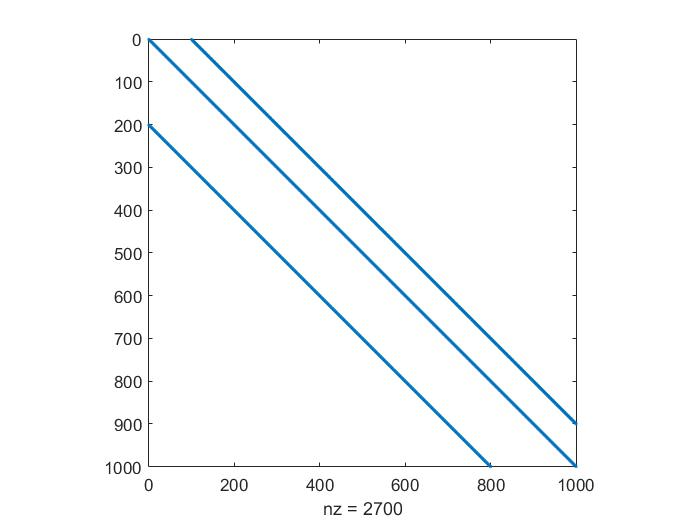
\includegraphics[scale=0.3]{example1.jpg}
\caption{$k=200$ and $l=100$}
\end{figure}

\begin{thm}[General case]
The upper triangular matrix $R$ in the $QR$ decomposition of $A$ has a $k+l$-band structure.
\end{thm}
\begin{proof}
From the CGS method we immediately see, in the worst case, the first $j+k$ entries are non zero.
Therefore, the inner product in the computation of the entries $r_{ij}$ is only zero if $i<j-l-k+2$. 
\end{proof}
\indent To illustrate this, consider the example of a matrix close to the worst case, where the number of non-zero entries (nz) increases by order 50:
\begin{figure}[H] 
    \subfigure[A]{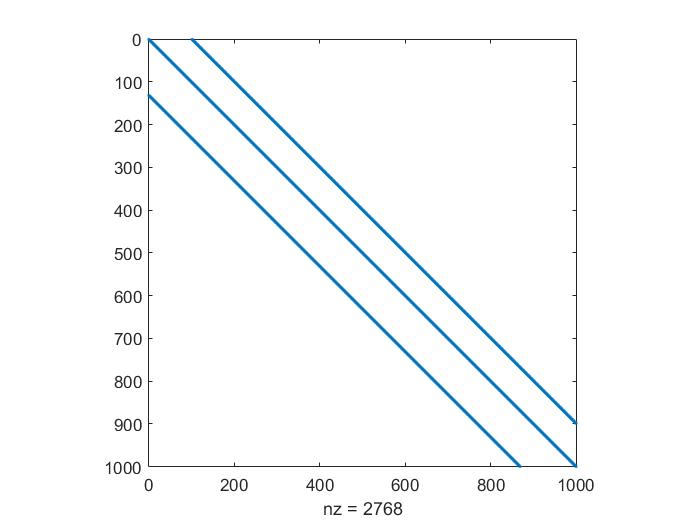
\includegraphics[width=0.49\textwidth]{example2.jpg}} 
    \subfigure[R]{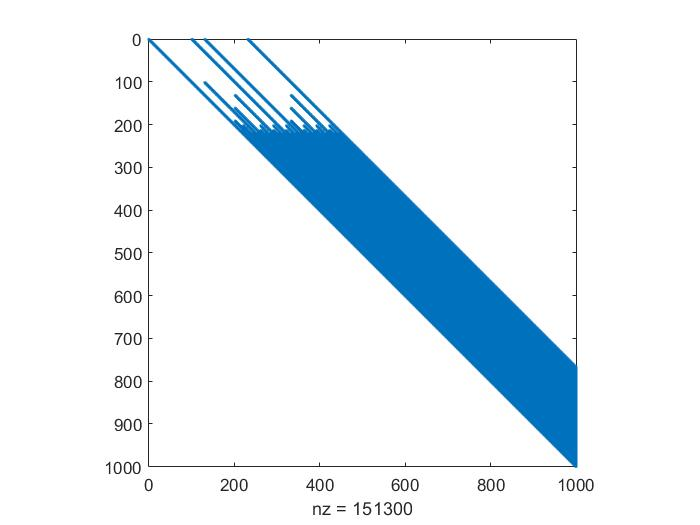
\includegraphics[width=0.49\textwidth]{example3.jpg}}  

    \caption{$k=131$ and $l=101$}
\end{figure} 
\indent A special case occurs when $k=l$. Again, $R$ has only three non-zero bands: the main diagonal, the superdiagonal that has a distance $k$ to the main diagonal, and the superdiagonal that has a distance $2k$ to the main diagonal. For $k = l = 100$:
\begin{figure}[H] 
    \subfigure[A]{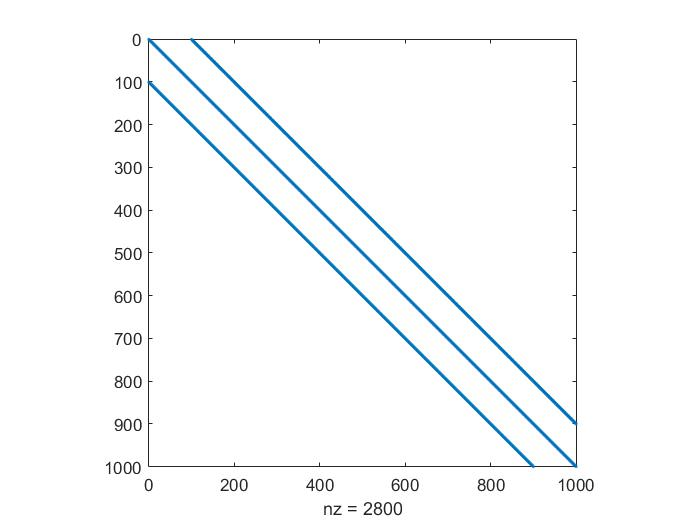
\includegraphics[width=0.49\textwidth]{example4.jpg}} 
    \subfigure[R]{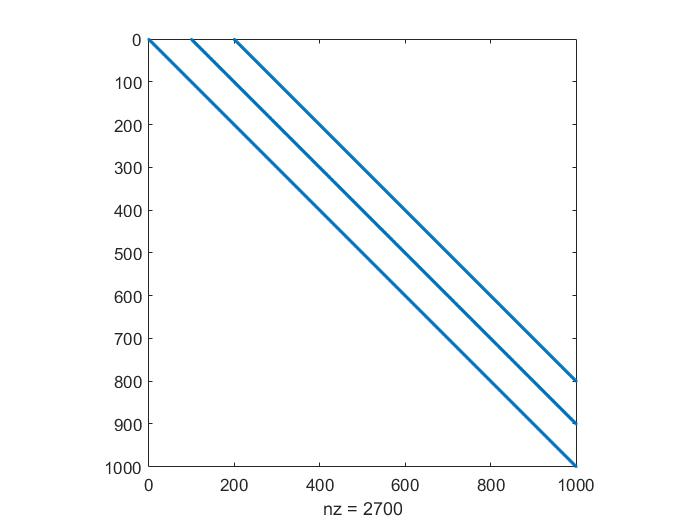
\includegraphics[width=0.49\textwidth]{example5.jpg}}  

    \caption{$k=l=100$ }
\end{figure} 
\section{Algorithms and Results}
\indent Based on the properties proved in section 2, it is fairly straightforward
to modify existing algorithms for finding the QR-factorization of a matrix, to
exploit sparsity patterns.
\subsection{General Banded Matrices}
\indent Suppose $A\in C^{m\times n}$ with bandwidth $2p +1$. Consider the QR-factorization
of $A$, $A = QR$. Then by Theorem 2.2, we
know that if $j > i + 2p$, $r_{ij} = 0$. We can alter the well-known
\textit{Modified Gram-Schmidt} (MGS) algorithm to take advantage of this fact,
as shown below.
\begin{algorithm}[H]
  \caption{MGS for Banded Matrices [Banded MGS]}
  \begin{algorithmic}[1]
    \For{$i = 1$\textbf{ to }$n$}
    \State$r_{ii}\gets \norm{\mathbf{a_i}}_2$
    \State$q_i\gets \mathbf{a_i} / r_{ii}$
    \For{$j = i + 1$\textbf{ to }$\text{min}\set{i + 2p, n}$}
    \State$r_{ij}\gets \mathbf{q_i}^*\mathbf{a_j}$
    \State$\mathbf{v_j}\gets\mathbf{v_j} - r_{ij}\mathbf{q_i}$
    \EndFor
    \EndFor
  \end{algorithmic}
  [Note that this is based on the \textit{Modified
    Gram-Schmidt} algorithm as described in \cite{nla}] 
\end{algorithm}
\indent We will examine the performance of \textbf{Algorithm 1} later, but first we will
examine more specific cases which allow for further optimization.
\subsection{Special Cases}
\indent In the special case of the symmetric tridiagonal matrix $A$, where the super and sub diagonal have a distance $k$ from the diagonal, we can improve the \textbf{Algorithm 1} even further using \textbf{Theorem} and \textbf{Corollary}.
\begin{algorithm}[H]
  \caption{MGS for special tridiagonal Matrices }
  \begin{algorithmic}[1]
    \For{$i = 1$\textbf{ to }$n$}
   	\State$v_i\gets a_i$
    \EndFor
    \For{$i = 1$\textbf{ to }$n$}
    \State$r_{ii}\gets \norm{\mathbf{v_i}}_2$
    \State$q_i\gets \mathbf{v_i} / r_{ii}$ 
    \If{$i+2k+2\leq n$}
    	\State$r_{i,i+2k+2}\gets \mathbf{q_i}^*\mathbf{a_{i+2k+2}}$
    	\State$\mathbf{v_{i+2k+2}}\gets\mathbf{v_{i+2k+2}} - r_{i,i+2k+2}\mathbf{q_i}$
    	\State$r_{i,i+k+}\gets \mathbf{q_i}^*\mathbf{a_{i+k+1}}$
    	\State$\mathbf{v_{i+k+1}}\gets\mathbf{v_{i+k+1}} - r_{i,i+k+1}\mathbf{q_i}$
    	\ElsIf{$i+k+1\leq n$}
    	\State$r_{i,i+k+}\gets \mathbf{q_i}^*\mathbf{a_{i+k+1}}$
    	\State$\mathbf{v_{i+k+1}}\gets\mathbf{v_{i+k+1}} - r_{i,i+k+1}\mathbf{q_i}$
       	\EndIf
    \EndFor
  \end{algorithmic}
\end{algorithm}
\subsection{Flop count}
\indent Here, we are going to give the theoretical flop count of the two algorithms and compare it with the MGS algorithm in \cite{nla}.\\
\indent Recall that the MGS requires $\sim 2n^3$ operations, where the most amount of work is due to an inner \textit{for}-loop.
In both of the above algorithms we can eliminate/ heavily reduce the the size of the inner \textit{for}-loop.
Therefore the first algorithm has a flop count of $\sim 8*2pn^2$ and the second
one for the special case tridiagonal matrices we have $\sim 8n^2$ flops.
\subsection{Case Study}
\indent To test the performance of \textbf{Algorithm 1} in a real-world
computing setting, we wrote version of it in \texttt{Matlab/Octave} and ran it
on a \textit{Raspberry Pi 3}, timing its performance on random banded matrices versus
the performance of the MGS algorithm. For actual code and raw data, please see
the appendix.\\
\indent Below is a table of ratios 
\begin{equation*}
  \Frac{\text{Banded MGS time}}{\text{MGS time}}
\end{equation*}
for square random banded matrices of increasing dimensions and bandwidths.
\begin{center}
  \begin{tabular}{|| c || c | c | c | c | c | c ||}
    \hline
    $m / p$ & $0$ & $\frac{m}{10}$ & $\frac{m}{5}$ & $\frac{3m}{10}$ & $\frac{2m}{5}$ & $\frac{m}{2}$\\
    \hline\hline
    10 & 0.243 & 0.577 & 0.799 & 0.952 & 1.040 & 1.055\\
    \hline
    500 & 0.006 & 0.365 & 0.644 & 0.844 & 0.961 & 1.006\\
    \hline
750 & 0.004 & 0.364 & 0.641 & 0.839 & 0.959 & 1.001\\
    \hline
1000 & 0.003 & 0.363 & 0.644 & 0.841 & 0.964 & 1.000\\
    \hline
  \end{tabular}
\end{center}
\indent These results seem to agree with our intuitive understanding of how
\textbf{Algorithm 1} provides benefits for banded matrices. It is clear that as
the bandwidth increases, the run times for Banded MGS and MGS converge, i.e. as
$p$ gets closer to $m$, we see no real improvement. This agrees with our flop
count above, since if $p\approx m$, the flop count of \textbf{Algorithm 1} is
$\sim 8pm^2\approx 8m^3\sim m^3$, which is the performance we expect from the standard
MGS algorithm. We also can see less speedup for the case where the given matrix
is in $\R^{10\times 10}$, but this may just be because the effect of optimizations are
generally more apparent in extreme cases, and a $10\times 10$ matrix is
certainly not that.
\indent Below is a plot demonstrating the run times for the Banded
MGS Algorithm versus the MGS algorithm on random $1000\times 1000$ matrices with
increasing bandwidth (from the same dataset as the table above).
\begin{center}
  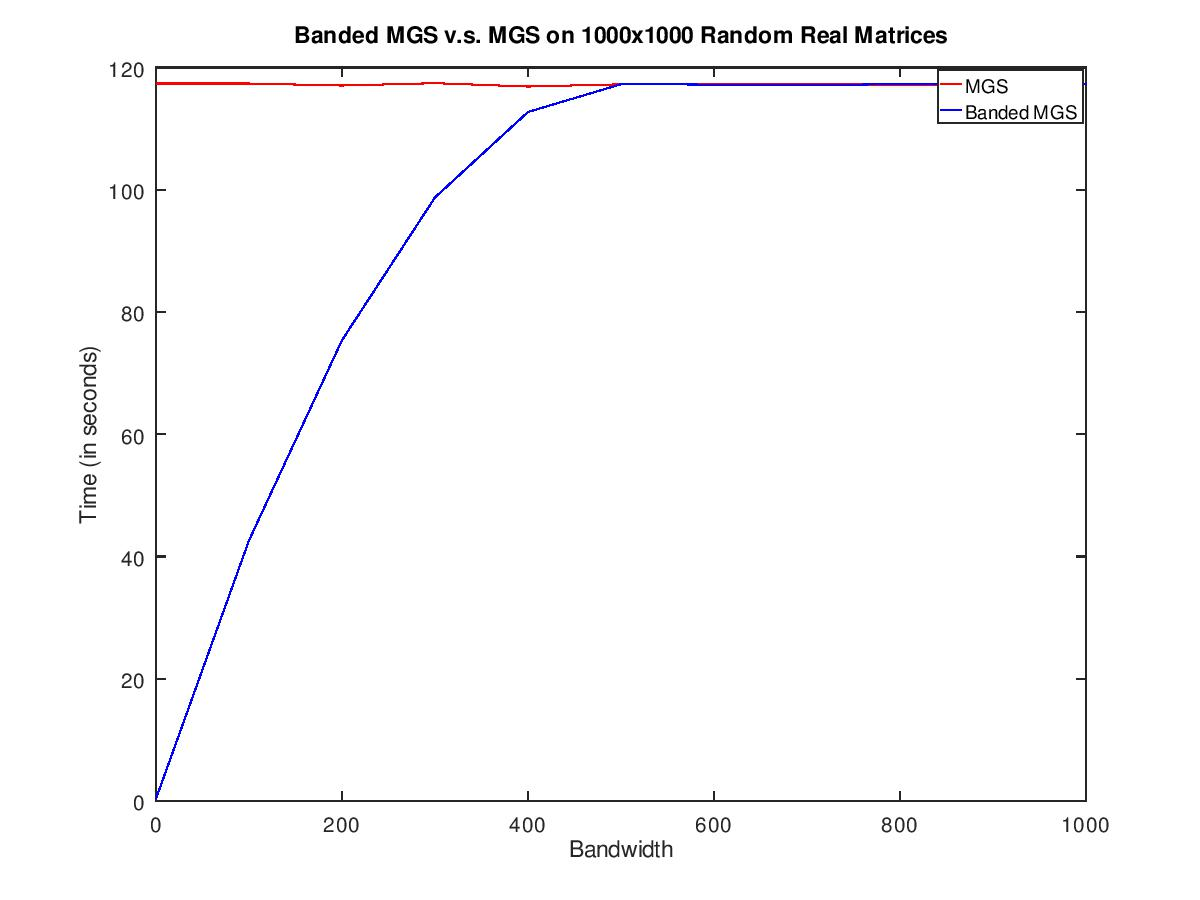
\includegraphics[scale=0.4]{pi-data.jpg}
\end{center}
\section{Further Study}
\indent There are several avenues for future work on this topic. Other
algorithms, such as Householder triangularization, may be able to take advantage
of the properties of banded matrices and address the poor stability of Modified
Gram-Schmidt. Our report also never considers memory optimization with the use
of a compressed storage format, such as Compressed Sparse Row (CSR) or diagonal
form. Finally, further work may investigate the application of banded matrix
properties to algorithmic parallelization of Modified Gram-Schmidt and other
algorithms.
\appendix
\addcontentsline{toc}{section}{Appendix}
\section*{Appendix}
All raw data and source code referenced in this paper can be found on
GitHub at
\begin{center}
  \href{https://github.com/drVulter/comp-math-project}{\texttt{https://github.com/drVulter/comp-math-project}}
\end{center}
	\addcontentsline{toc}{section}{References}
	\bibliographystyle{unsrt}
\bibliography{comp-math}
\end{document}